% interactcadsample.tex
% v1.03 - April 2017

\documentclass[]{interact}

\usepackage{epstopdf}% To incorporate .eps illustrations using PDFLaTeX, etc.
\usepackage{subfigure}% Support for small, `sub' figures and tables
%\usepackage[nolists,tablesfirst]{endfloat}% To `separate' figures and tables from text if required

\usepackage{natbib}% Citation support using natbib.sty
\bibpunct[, ]{(}{)}{;}{a}{}{,}% Citation support using natbib.sty
\renewcommand\bibfont{\fontsize{10}{12}\selectfont}% Bibliography support using natbib.sty

\theoremstyle{plain}% Theorem-like structures provided by amsthm.sty
\newtheorem{theorem}{Theorem}[section]
\newtheorem{lemma}[theorem]{Lemma}
\newtheorem{corollary}[theorem]{Corollary}
\newtheorem{proposition}[theorem]{Proposition}

\theoremstyle{definition}
\newtheorem{definition}[theorem]{Definition}
\newtheorem{example}[theorem]{Example}

\theoremstyle{remark}
\newtheorem{remark}{Remark}
\newtheorem{notation}{Notation}


% tightlist command for lists without linebreak
\providecommand{\tightlist}{%
  \setlength{\itemsep}{0pt}\setlength{\parskip}{0pt}}



\usepackage{hyperref}
\usepackage[utf8]{inputenc}
\def\tightlist{}
\usepackage{setspace}


\begin{document}


\articletype{Short Technical Note}

\title{A new simplified manual tour, with examples in mathematica}


\author{\name{Alex Aumann$^{a}$, German Valencia$^{a}$, Ursula
Laa$^{b}$, Dianne Cook$^{c}$}
\affil{$^{a}$School of Physics and Astronomy, Monash
University; $^{b}$Institute of Statistics, University of Natural
Resources and Life Sciences, Vienna; $^{b}$Department of Econometrics
and Business Statistics, Monash University}
}

\thanks{CONTACT Alex
Aumann. Email: \href{mailto:aaum0002@student.monash.edu}{\nolinkurl{aaum0002@student.monash.edu}}, German
Valencia. Email: \href{mailto:german.valencia@monash.edu}{\nolinkurl{german.valencia@monash.edu}}, Ursula
Laa. Email: \href{mailto:ursula.laa@boku.ac.at}{\nolinkurl{ursula.laa@boku.ac.at}}, Dianne
Cook. Email: \href{mailto:dicook@monash.edu}{\nolinkurl{dicook@monash.edu}}}

\maketitle

\begin{abstract}
Something here
\end{abstract}

\begin{keywords}
data visualisation; grand tour; statistical computing; statistical
graphics; multivariate data; dynamic graphics
\end{keywords}

\hypertarget{introduction}{%
\section{Introduction}\label{introduction}}

From a statistical perspective it is rare to have data that are strictly
3D, and so unlike in most computer graphics applications, the more
useful methods for data analysis show projections from an arbitrary
dimensional space. These are dynamic data visualizations methods and are
collected under the term \emph{tours}. Tours involve views of
high-dimensional (\(p\)) data in low-dimensional (\(d\)) projections. In
his original paper on the grand tour, \citet{As85} provided several
algorithms for tour paths that could theoretically show the viewer the
data \emph{from all sides}. Prior to Asimov's work, there were numerous
preparatory developments including \citet{tukey}'s PRIM-9. PRIM-9 had
user-controlled rotations on coordinate axes, allowing one to manually
tour through low-dimensional projections. It is impractical to
impossible to steer through all possible projections, unlike Asimov's
tours which allows one to quickly see many, many different projections.
After Asimov there have been many, many tour developments, as summarized
in \citet{lee2021}.

One such direction of work develops the ideas from PRIM-9, to provide
manual control of a tour. \citet{cook_manual_1997} describes controls
for 1D (or 2D) projections, in a 2D (or 3D) manipulation space, allowing
the user to select any variable axis, and rotate it into or out of or
around the projection through horizontal, vertical, oblique, radial or
angular changes in value. \citet{spyrison_spinifex_2020} refines this
algorithm and implements them to generate animations.

Manual controls are especially useful for assessing sensitivity of
structure to particular elements of the projection. There are many
places where it is useful. In exploratory data analysis, where one sees
clusters in a projection, can some variables be removed from the
projection without affecting the clustering. For interpreting models,
one can reduce or increase a variable's contribution to examine the
variable importance. These controls can also be used to interactively
generate facetted plots \citep{XXX}, or spatiotemporal glyphmaps
\citep{XXX}. Having the user interact with a projection is extremely
valuable for understanding high-dimensional data. However, these
algorithms have two problems: (1) the pre-processing of creating a
manipulation space overly complicates the algorithm, (2) extending to
higher dimensional control is difficult.

Through experiments with the relatively new interactive graphics
capabilities in mathematica(?), we have realized that there is a simpler
approach, which is more direct, and extensible for generating user
interaction. This paper explains this, and is organized as follows. The
next section describes the new algorithm for manual control. This is
followed by details on implementation. The applications section
illustrate how these can be used.

\hypertarget{sec:method}{%
\section{Manual tour}\label{sec:method}}

\hypertarget{background}{%
\subsection{Background}\label{background}}

Describe the manip space, out of manual tour

\hypertarget{new-definition}{%
\subsection{New definition}\label{new-definition}}

\begin{enumerate}
\def\labelenumi{\arabic{enumi}.}
\tightlist
\item
  Provide a k-D projection
\item
  Select variable to control
\item
  Detect or provide direction of change
\item
  Update projection, and orthonormalise
\end{enumerate}

Need to think about how the values for selected variable are made exact,
that is constrained orthonormalisation.

Need to think about checks, and error catching, maybe in implementation
section. If selected variable has 0 coefficient, will that generate an
orthonormalisation error?

\begin{figure}
\centering
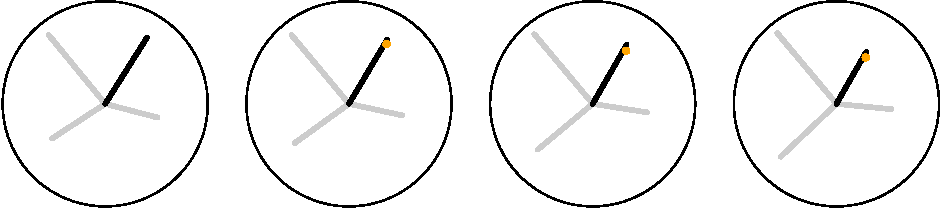
\includegraphics{paper_files/figure-latex/manualsequence-1.pdf}
\caption{Sequence of projections where V3 contribution is changed.}
\end{figure}

\hypertarget{sec:implementation}{%
\section{Implementation}\label{sec:implementation}}

\hypertarget{sec:examples}{%
\section{Applications}\label{sec:examples}}

\hypertarget{sec:discussion}{%
\section{Discussion}\label{sec:discussion}}

\hypertarget{acknowledgements}{%
\section*{Acknowledgements}\label{acknowledgements}}
\addcontentsline{toc}{section}{Acknowledgements}

The authors gratefully acknowledge the support of the Australian
Research Council. The paper was written in \texttt{rmarkdown}
\citep{rmarkdown} using \texttt{knitr} \citep{knitr}.

\hypertarget{supplementary-material}{%
\section*{Supplementary material}\label{supplementary-material}}
\addcontentsline{toc}{section}{Supplementary material}

The source material and animated gifs for this paper are available at

\bibliographystyle{tfcad}
\bibliography{biblio.bib}





\end{document}
